\chapter{Resultados}
\label{ch:07}

O enfoque deste capítulo será em analisar os resultados obtidos pelos experimentos com o modelo encoder-decoder.   

\begin{itemize}
    \item explicar que nessa seção vou analisar os resultados obtidos
    \item introduzir que a acurácia nao foi muito boa e que apesar disso tento entender os resultados dos modelos
    \item falar sobre a dificuldade de interpretação dos resultados de modelos de redes neurais
    \item falar sobre os poucos dados disponíveis%(https://medium.com/scribd-data-science-engineering/experiments-with-seq2seq-data-dependency-62184993f555)
\end{itemize}

\section{Treinamento}

\begin{itemize}
    \item Explicar o que são épocas
    \item explicar o que é batch size
    \item explicar hiperparâmetros
\end{itemize}
\subsection{300 epochs}
\begin{figure}[H]
  \centering
  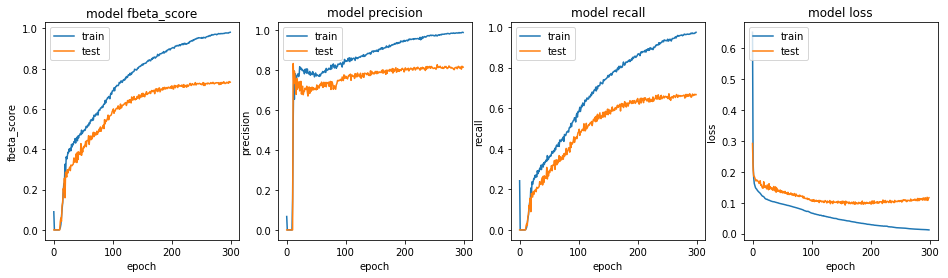
\includegraphics[width=1.0\linewidth]{img/300_fbeta.png}
  \caption{Resultados 300 epocas}
  \label{fig:training}
\end{figure}

Explicar as metricas em analise:
\begin{itemize}
    \item o que representa o f score
    \item o que representa a precision
    \item recall
    \item erro
    \item explicar pq as metricas parecem muito boas
\end{itemize}
\subsection{2000 epochs}


\begin{figure}[H]
  \centering
  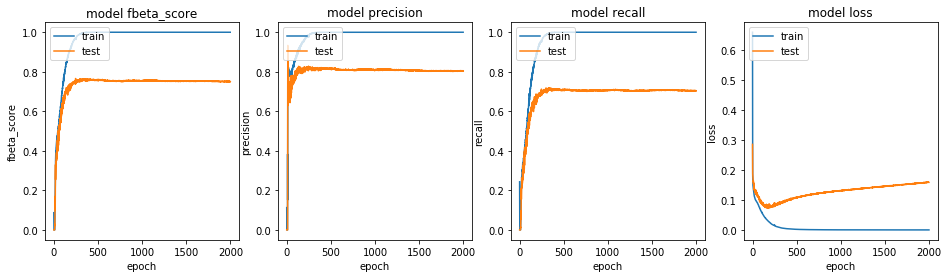
\includegraphics[width=1.0\linewidth]{img/2000_precision.png}
  \caption{Resultados 2000 Epocas}
  \label{fig:encdec}
\end{figure}

Mostrar aonde começa o overfit e discutir que 300 epocas era o suficiente

\section{Análise K-Fold}

Como o tamanho do corpus disponível é restrito, não é interessante realizar um único experimento com uma única segmentação entre treino e teste, pois haveriam verbos em que o modelo nunca seria testado e outros que nunca seriam utilizados no treinamento. Dessa forma a acurácia do modelo poderia variar bastante dependendo dos verbos sorteados para cada um desses grupos. Assim, uma técnina de validação cruzada chamada \textit{K-Fold} foi escolhida para o estudo dos resultados. A análise K-Fold permite que o modelo seja avaliado em todos os verbos do corpus. A técnica consiste, primeiramente, na formação de K subconjuntos de verbos mutuamente exclusivos de mesmo tamanho. Em seguida, um desses subconjuntos é escolhido como o conjunto de teste enquanto que os K-1 restantes são utilizados como treino. O tamanho de K é definido a partir da escolha de proporção em que se deseja realizar a segmentação entre treino e teste, ou seja, para sempre manter a proporção de testes em 20\% de modo que estes verbos sejam sempre diferentes, o corpus precisa ser segmentado em 5 subconjuntos distintos. O desenho ref{desenho} ilustra o algoritmo. 

desenho

Além disso, há ainda uma outra restrição que essa análise contempla. Ela permite que em cada um desses treinamentos, as proporções das classes de verbos se mantenham no treinamento. Isso significa que, por exemplo, a classe de irregularidades 12 (testar -> tEstu) que possui 20 verbos, terá sempre 16 verbos verbos no treinamento e 4 no teste. Assim, após os 5 treinamentos difernetes, todos os verbos da classe foram testados e há a certeza de que haviam verbos dessa classe no treinamento.








\begin{figure}[H]
  \centering
  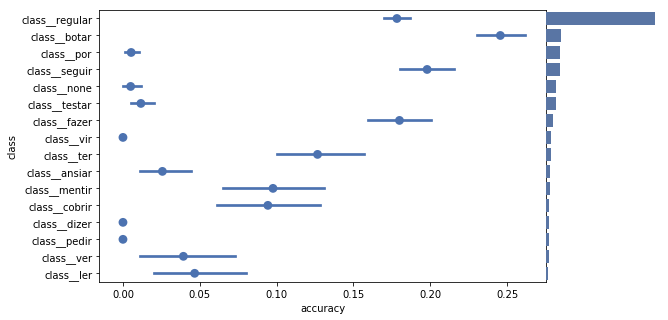
\includegraphics[width=1.0\linewidth]{img/accuracy_kfold_1.png}
  \caption{Acuracia kfold com desvio padrao ordenada por proporcao da classe}
  \label{fig:kfoldprop}
\end{figure}

Falar sobre o grafico e tentar entender porque a familia do verbo "botar" obteve mais sucesso que as outras. Há relacao de proporção da familia com perplexidade ou tamanho medio dos verbos?

Falar sobre a perplexidade das familias de verbos.

\begin{table}[]
\centering
\begin{tabular}{ll}
Classe  & Perplexidade \\
\toprule
Regular & 1.00366      \\
\hline
Por     & 1.02165      \\
\hline
Seguir  & 1.02730      \\
\hline
Botar   & 1.03139      \\
\hline
Testar  & 1.03663      \\
\hline
Fazer   & 1.04015      \\
\hline
None    & 1.04198      \\
\hline
Vir     & 1.060829     \\
\hline
Ansiar  & 1.073437     \\
\hline
Ter     & 1.073437     \\
\hline
Mentir  & 1.089055     \\
\hline
Dizer   & 1.094539     \\
\hline
Pedir   & 1.115955     \\
\hline
Ver     & 1.115955     \\
\hline
Cobrir  & 1.118949     \\
\hline
Ler     & 1.172332    \\
\bottomrule
\end{tabular}
\caption{Classes de Irregularidades Ordenadas por Perplexidade}
\label{tab:perplexity}
\end{table}


\begin{figure}[H]
  \centering
  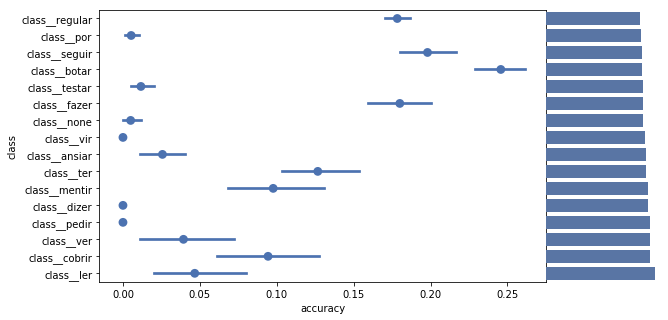
\includegraphics[width=1.0\linewidth]{img/accuracyperplexity.png}
  \caption{Acuracia por Perplexidade Ascendente}
  \label{fig:kfoldprop}
\end{figure}

Falar sobre o tamanho médio dos verbos alvo.

\begin{figure}[H]
  \centering
  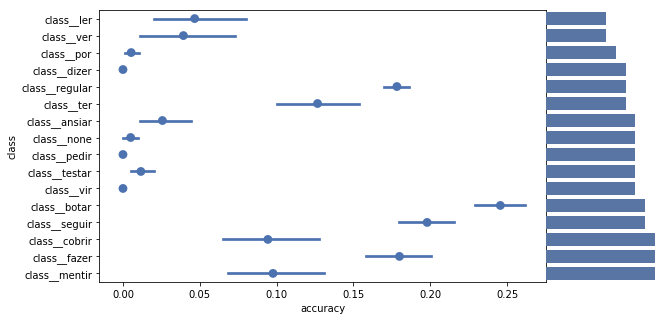
\includegraphics[width=1.0\linewidth]{img/downloadaccuracy_kfold_3.png}
  \caption{Acuracia por Cumprimento Medio Ascendente}
  \label{fig:kfoldprop}
\end{figure}


\section{Análise dos Erros}

Falar que eu escolhi o arquivo com a maior acuracia para analisar. Esse arquivo teve um total de 73 acertos, 17\% de acuracia.


\section{Arquivo com melhores resultados}

\begin{figure}[H]
  \centering
  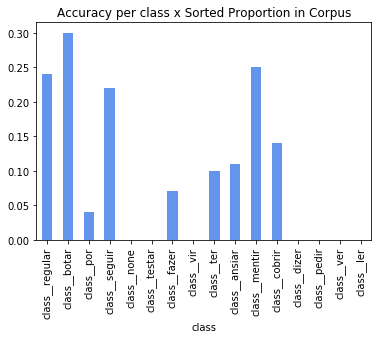
\includegraphics[width=0.7\linewidth]{img/best_file_accuracy.png}
  \caption{Acuracia proporcao corpus}
  \label{fig:acuraciaprop}
\end{figure}



\begin{figure}[H]
  \centering
  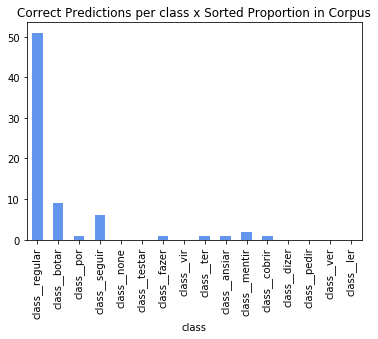
\includegraphics[width=0.7\linewidth]{img/best_file_correct_p.png}
  \caption{Predicoes corretas x proporcao}
  \label{fig:predicxprop}
\end{figure}

\begin{figure}[H]
  \centering
  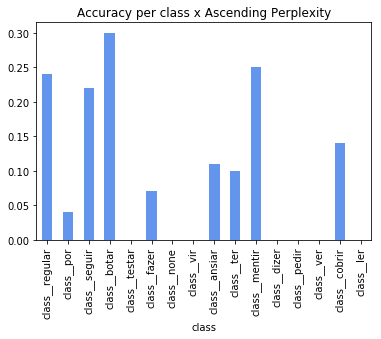
\includegraphics[width=0.7\linewidth]{img/best_file_acuracy_perplexity.png}
  \caption{acuracia perplexidade}
  \label{fig:acuper}
\end{figure}

\begin{figure}[H]
  \centering
  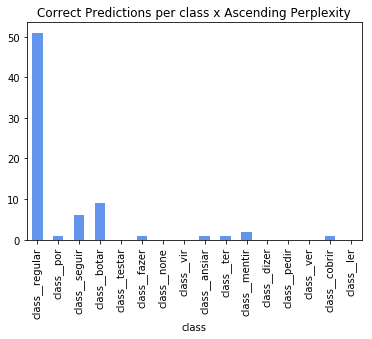
\includegraphics[width=0.7\linewidth]{img/best_file_accuracy_perplexity.png}
  \caption{prediçoes corretas x perplexidade}
  \label{fig:prexper}
\end{figure}


mostrar uma tabela com esse arquivo e analisar os erros encontrados

discussao dos resultados
cada classe
comentar sobre erros interessantes, por exemplo trocas de classes
experimentos com verbos inventados
